\documentclass[border=6pt]{standalone}
\usepackage{tikz}
\usetikzlibrary{arrows.meta,calc}
\begin{document}
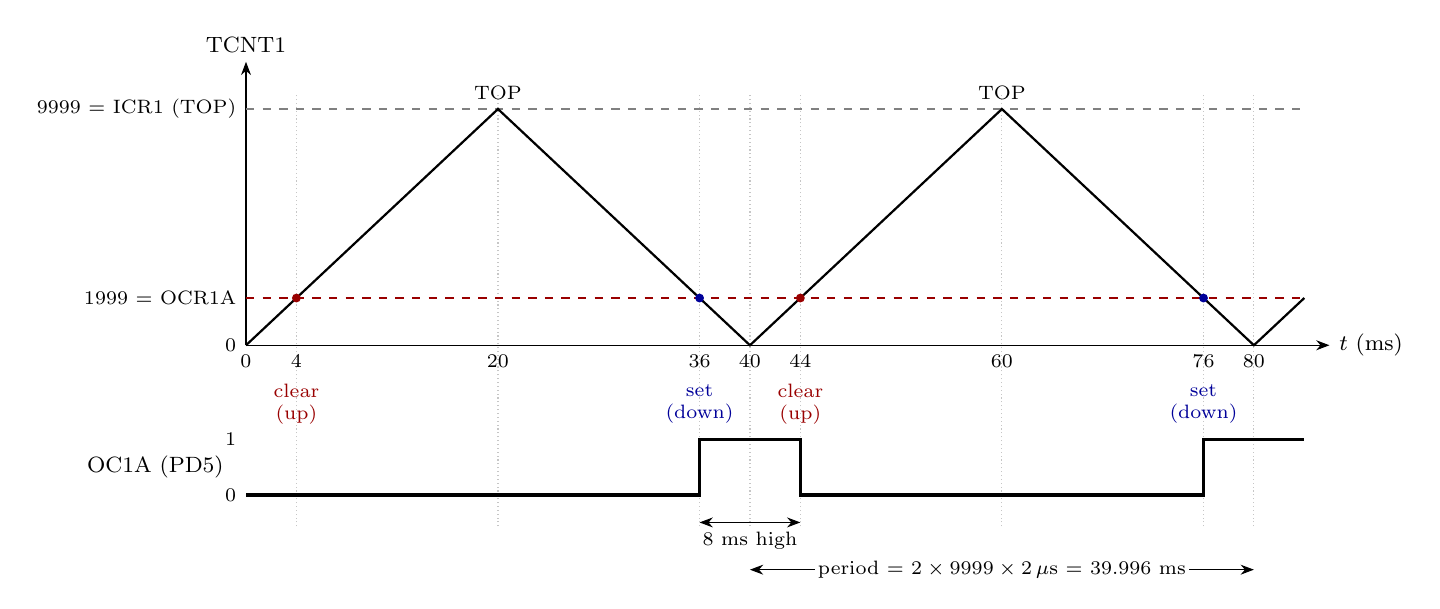
\begin{tikzpicture}[>=Stealth,font=\small,x=0.16cm,y=1cm]
% 1 unit = 1 ms; 1 tick = 2 us; TOP = 9999 reached at 19.998 ms, BOTTOM at 39.996 ms
\def\H{3.0}% TOP = 9999
\def\C{0.5998}% OCR1A = 1999 -> 3.0*1999/9999
\foreach \t in {4,20,36,40,44,60,76,80} \draw[gray!45,densely dotted] (\t,-2.3) -- (\t,\H+0.2);
\draw[->] (0,0) -- (0,\H+0.6) node[above,font=\footnotesize]{TCNT1};
\draw[->] (0,0) -- (86,0) node[right,font=\footnotesize]{$t$ (ms)};
\node[anchor=east,font=\scriptsize] at (0,\H) {9999 = ICR1 (TOP)};
\node[anchor=east,font=\scriptsize] at (0,\C) {1999 = OCR1A};
\node[anchor=east,font=\scriptsize] at (0,0) {0};
\draw[gray,dashed] (0,\H) -- (84,\H);
\draw[red!60!black,dashed] (0,\C) -- (84,\C);
\draw[thick] (0,0) -- (20,\H) -- (40,0) -- (60,\H) -- (80,0) -- (84,0.6);
\foreach \t in {4,44} \fill[red!60!black] (\t,\C) circle (1.6pt);
\foreach \t in {36,76} \fill[blue!60!black] (\t,\C) circle (1.6pt);
\foreach \t in {0,4,20,36,40,44,60,76,80} \node[below,font=\scriptsize] at (\t,0) {\t};
\node[font=\scriptsize,above,align=center] at (20,\H) {TOP};
\node[font=\scriptsize,above,align=center] at (60,\H) {TOP};
% OC1A
\begin{scope}[yshift=-1.9cm]
\node[anchor=east,font=\footnotesize] at (-1,0.35) {OC1A (PD5)};
\node[anchor=east,font=\scriptsize] at (0,0.7) {1};
\node[anchor=east,font=\scriptsize] at (0,0) {0};
\draw[very thick] (0,0) -- (36,0) -- (36,0.7) -- (44,0.7) -- (44,0) -- (76,0) -- (76,0.7) -- (84,0.7);
\node[font=\scriptsize,red!60!black,align=center] at (4,1.15) {clear\\(up)};
\node[font=\scriptsize,blue!60!black,align=center] at (36,1.15) {set\\(down)};
\node[font=\scriptsize,red!60!black,align=center] at (44,1.15) {clear\\(up)};
\node[font=\scriptsize,blue!60!black,align=center] at (76,1.15) {set\\(down)};
\draw[<->] (36,-0.35) -- (44,-0.35) node[midway,below,font=\scriptsize]{8 ms high};
\draw[<->] (40,-0.95) -- (80,-0.95) node[midway,fill=white,font=\scriptsize,inner sep=1pt]{period = $2\times9999\times2\,\mu$s = 39.996 ms};
\end{scope}
\end{tikzpicture}
\end{document}
